\section{Setup}
In this section, we will explain how to get Germinate 3 up and running.

\subsection{Requirements}
We try to keep the requirements of Germinate 3 as basic as possible. In order to run Germinate 3 you will need to have the following applications available on your server:

\begin{itemize}
	\item \textit{Apache Tomcat} (7.0.28 or above) to run the web application
	\item \textit{Java} (8 or above) to run Apache Tomcat and the Germinate 3 server side code
	\item \textit{MySQL} (or \textit{MariaDB}) (5.6.1 or above) database to hold the data
	\item \textit{Apache Ant} (1.9.1 or above) to compile to \texttt{.war} files
\end{itemize}
\noindent
Please make sure that you have the required applications installed before continuing.

\subsection{Configuration of Apache Tomcat}
\textit{If you already have a Tomcat user account, skip this step.}\\
\\
Once Apache Tomcat is installed, you will need to create a user account. This user account will be used to deploy Germinate 3 to Tomcat. To add a user account, open the file \texttt{<Tomcat Directory>/conf/tomcat-users.xml} and add the following line:

\begin{lstlisting}[style=Xml]
<user username="<Username>" password="<Password>" roles="manager-gui,manager-script"/>
\end{lstlisting}
\noindent
Just replace the username and password placeholders with the credentials you want to use. Tomcat needs to be restarted after these two steps. Remember the username and password, we will need them later.

\subsection{Germinate and Gatekeeper databases}
\todo{Explain how to create initial databases.}

\subsection{Configuration of MySQL}
\label{sec:mysql-basic}
\textit{If you already have a MySQL user account that has permissions to query the Germinate 3 and Germinate Gatekeeper databases, skip this step.}\\
\\
After the installation of MySQL, you need to create a user account for Germinate 3, so that the web application can query the database. Remember the username and password, we will need them later.

Once the user is created, you can grant permissions to the newly created user. It is save to grant this user all available permissions for the Germinate 3 and Germinate Gatekeeper database. The minimal set of required permissions are: \texttt{select}, \texttt{insert}, \texttt{delete}, \texttt{update}, \texttt{create view}, \texttt{create routine} and \texttt{execute}.

\subsection{Basic setup}
In the best case, you already have a compiled version of Germinate 3 and Germinate Gatekeeper in the form of a \texttt{.war} file each as well as their database counterparts in your MySQL installation. 

\begin{figure}
	\centering
	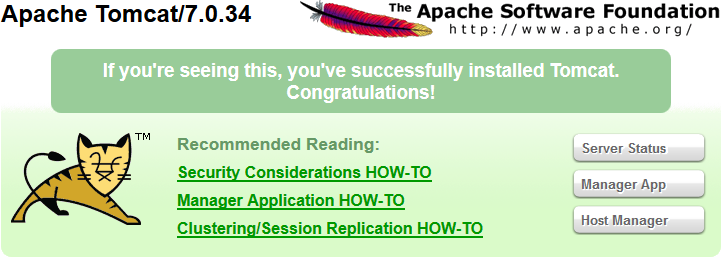
\includegraphics[scale=0.5]{img/setup/tomcat.png}
	\caption{Tomcat welcome screen}
	\label{fig:tomcat}
\end{figure}
\noindent
To deploy these applications, navigate to the following URL:
\begin{center}
	\texttt{http://<Your web server>:8080}
\end{center}
You should see something similar to Figure \ref{fig:tomcat}. Click on the button labelled "Manager App" and you will be prompted to enter your credentials. Use the username and password defined in the file \texttt{tomcat-users.xml}. The following page will show all the applications running on Tomcat right now. Below this table, there is a section called "Deploy" with subsection "WAR file to deploy". Simply select each of the two WAR files by clicking on the "Browse" button and then click on "Deploy". Germinate 3 and Gatekeeper should now be listed in the applications table at the top of the page.

Clicking on the \texttt{Path} link in the first column of the overview table should redirect you to Germinate 3 and Germinate Gatekeeper respectively.

\subsection{Advanced setup}
In this section, we will explain how you compile Germinate 3 (Germinate Gatekeeper analogously) from source. This is required if you do not have pre-compiled versions of the applications. We will also explain how you can create empty versions of the Germinate 3 and Germinate Gatekeeper databases in your database server.

\subsubsection{Download of source code}

First, download the Germinate 3 and Germinate Gatekeeper source code from our SVN:

\begin{itemize}
	\item Germinate 3
	\begin{itemize}
		\item \url{https://ics.hutton.ac.uk/svn/germinate3}
	\end{itemize}
	\item Germinate Gatekeeper
	\begin{itemize}
		\item \url{https://ics.hutton.ac.uk/svn/germinate-gatekeeper}
	\end{itemize}
\end{itemize}

\subsubsection{Configuration of source code}
\label{sec:germinate-config}
Both applications contain a file called \texttt{build.xml} which is the Apache Ant build script as well as an associated \texttt{build.properties} file. These files are used to compile and deploy the application.

Edit the \texttt{build.properties} file and replace the placeholder username and password with your Apache Tomcat username and password. Replace the placeholder for your web server as well.
\begin{lstlisting}[style=EclipseProperties]
# Ant properties for building the GWT app
project.name=germinate-templace
project.root=jhi.germinate.Germinate

instance.files=./(*\instanceStuff*)/template

tomcat.manager.url=http://<Your web server>:8080/manager/text
tomcat.manager.username=<Username>
tomcat.manager.password=<Password>
\end{lstlisting}
\noindent
The next file that needs editing is the \texttt{config.properties} file. In the case of Germinate Gatekeeper this file is located in the root directory. In the case of Germinate 3, you can find this file in the \texttt{\instanceStuff/<your germinate instance>} folder.\\
\\
Configure Germinate Gatekeeper in the following way:

\begin{lstlisting}[style=Properties]
database.server=<server holding germinate>
database.name=<database name>
database.useport=<is a port necessary?>
database.port=<port number>
database.username=<username, e.g. germinate3>
database.password=<password>
[...]
\end{lstlisting}
\noindent
Finally, configure Germinate 3 in the following way:

\begin{lstlisting}[style=Properties]
Germinate.Database.Server=<server holding germinate>
Germinate.Database.Name=<database name>
Germinate.Database.UsePort=<is a port necessary?>
Germinate.Database.Port=<port number>
Germinate.Database.Username=<username, e.g. germinate3>
Germinate.Database.Password=<password>

Gatekeeper.URL=<base url of gatekeeper>
Gatekeeper.Database.Name=<name of gatekeeper database>
Gatekeeper.Database.Server=<server holding gatekeeper>
Gatekeeper.Database.UsePort=<is a port necessary?>
Gatekeeper.Database.Port=<port number>
[...]
\end{lstlisting}

\subsubsection{Configuration of the database}

We've explained how to create a MySQL user account in Section \ref{sec:mysql-basic}. Now we will explain how to create empty versions of the Germinate 3 and Germinate Gatekeeper databases on your server.

Both application source folders contain a sub-folder called "database". This folder contains a \texttt{.sql} file that can be used to create an empty database (apart from default and required entries) for Germinate 3 and Germinate Gatekeeper respectively. Before you execute the scripts, make sure that you have an empty database per application that you can run the script against.

After running the two scripts, you should now have two template databases on your server. Grant your Germinate user access to those two databases. Make sure to grant at least the permissions listed in Section \ref{sec:mysql-basic}.

\subsubsection{Building the source code}
To build the application, simply run \texttt{ant} from the command line in the root directory of Germinate 3 and Germinate Gatekeeper. Apache Ant will then run the build script and compile the source code and finally deploy it to your Apache Tomcat installation.

Make sure that the machine you're compiling the source on can communicate with the web server via HTTP (required to deploy the application).

After the build finishes successfully, you should be able to view Germinate in your browser. The address is based on your configuration. It should have this structure: \texttt{http://<Your web server>:8080/<project.name>}.

\paragraph{Making code changes}
You are now free to change the code and add new pages. For examples of how to add new pages and other handy code snippets see Section \ref{sec:examples}.

\subsection{Germinate Gatekeeper Admin}
\label{subsection:gatekeeper-admin}

\begin{figure}
	\centering
	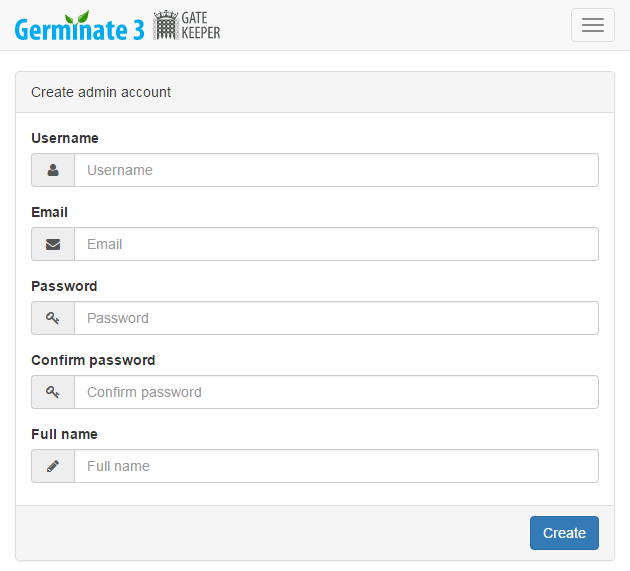
\includegraphics[scale=0.4]{img/setup/create-admin.png}
	\caption{Create admin account page}
	\label{fig:create-admin}
\end{figure}

The first time you go to the Germinate Gatekeeper website, you'll see the form shown in Figure \ref{fig:create-admin}. Fill it in to create the initial admin account. After this, you will be able to log in to Gatekeeper and create other users, database systems and set their permissions.

\subsection{Logging}
\label{subsection:logging}
Depending on your configuration (ref.\ \texttt{Germinate.Server.Logging.Enabled} in Section \ref{sec:config}), Germinate will log all server-side exceptions. This can be useful when you need to debug your version of Germinate.

The log files are stored to this location: \texttt{<Tomcat Directory>/temp/logs/}. Each instance of Germinate uses its own log files to avoid mix-ups.

\subsection{Docker}
Since version 3.3.1, a Germinate Demo Application is available as a Docker image. Please consult our website for more details:
\begin{center}
	\url{https://ics.hutton.ac.uk/germinate/germinate-docker-image}
\end{center}